\documentclass{beamer}
\usetheme{Warsaw}

\usepackage[utf8]{inputenc}
\usepackage{fancybox}
\usepackage{multimedia} 
\usepackage{subfig}
\usepackage{amsmath}
\usepackage{hyperref}
\usepackage{marvosym}

\usepackage[all]{xy}
\begin{document}


\title[Digitale Bildverarbeitung] % (optional, only for long titles)
{Digitale Bildverarbeitung
\\
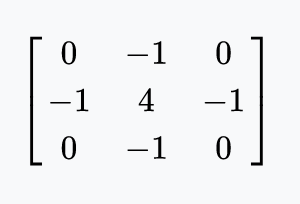
\includegraphics[scale=1.0]{img/cover}
}
\subtitle{}
\author[Dr. Johannes Riesterer] % (optional, for multiple authors)
{Dr.  rer. nat. Johannes Riesterer}

\date[KPT 2004] % (optional)
{}

\subject{Digitale Bildverarbeitung}

\frame{\titlepage}


\begin{frame}
    \frametitle{Morphologische Filter}
\framesubtitle{}

\begin{block}{Dilatation (binär)}
Sei $B \subset \mathbb{R}^n$ eine (nichtleere) Teilmenge und $u : \mathbb{R}^n \to \{ 0,1 \}$ eine binäres Bild.  Die Dilatation von $u$ mit dem Strukturelement $B$ ist definiert durch
\begin{align*}
(u \oplus B)(x) = \begin{cases} 1 \text{ falls für ein $y \in B$ gilt } u(x + y )= 1 \\ 0 \text{ sonst} \end{cases}
\end{align*}
\end{block}
\begin{figure}[htp]
      \centering
Dilatation eines Vierecks mit einem Kreis \\
    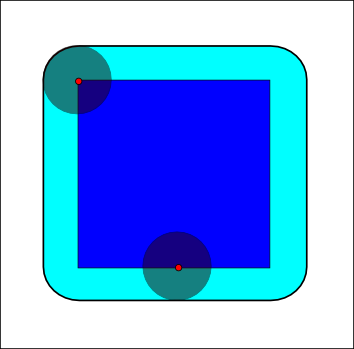
\includegraphics[width=0.25\textwidth]{img/Dilation} 
      \caption{Quelle: Wikipedia}
\end{figure}

 \end{frame}

\begin{frame}
    \frametitle{Morphologische Filter}
\framesubtitle{}

\begin{block}{Erosion (binär)}
Sei $B \subset \mathbb{R}^n$ eine (nichtleere) Teilmenge und $u : \mathbb{R}^n \to \{ 0,1 \}$  eine binäres Bild.  Die Erosion von $u$ mit dem Strukturelement $B$ ist definiert durch
\begin{align*}
(u \ominus B)(x) = \begin{cases} 1 \text{ falls für alle $y \in B$ gilt } u(x + y) = 1 \\ 0 \text{ sonst} \end{cases}
\end{align*}
\end{block}
\begin{figure}[htp]
      \centering
Erosion eines Vierecks mit einem Kreis \\
    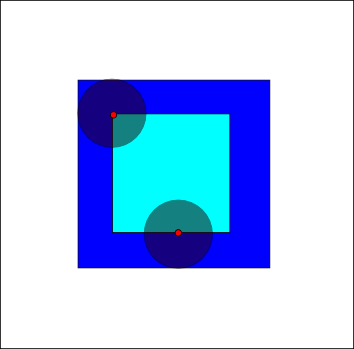
\includegraphics[width=0.25\textwidth]{img/Erosion} 
      \caption{Quelle: Wikipedia}
\end{figure}

 \end{frame}


\begin{frame}
    \frametitle{Morphologische Filter}
\framesubtitle{}

\begin{block}{Lemma}
Sei $B \subset \mathbb{R}^n$ eine (nichtleere) Teilmenge und $u : \mathbb{R}^n \to \{ 0,1 \}$. Dann gilt:
\begin{align*}
(u \oplus B)(x) = \sup_{y \in B} u(x +y) \\
(u \ominus B)(x) = \inf_{y \in B} u(x +y)
\end{align*}
\end{block}
\begin{block}{Beweis}
\begin{align*}
 \sup_{y \in B} u(x +y) = 1 \Leftrightarrow \exists y \in B: u(x +y) = 1  \\
\inf_{y \in B} u(x +y) = 1  \Leftrightarrow \forall y \in B: u(x +y) = 1  \\
\end{align*}
\end{block}

 \end{frame}


\begin{frame}
    \frametitle{Morphologische Filter}
\framesubtitle{}

\begin{block}{Dilatation und Erosion von Grauwertbildern}
Sei $B \subset \mathbb{R}^n$ eine (nichtleere) Teilmenge und $u : \mathbb{R}^n \to [ 0,1 ]$ ein kontinuierliches Grauwertbild. Dann ist die Dilatation und die Erosion definiert durch:
\begin{align*}
(u \oplus B)(x) =: \sup_{y \in B} u(x +y) \\
(u \ominus B)(x) := \inf_{y \in B} u(x +y)
\end{align*}
\end{block}

 \end{frame}


\begin{frame}
    \frametitle{Morphologische Filter}
\framesubtitle{}

\begin{block}{Diskretisierung morphologischer Operationen}
Sei $B \subset \mathbb{Z}^2$ eine (nichtleere) Teilmenge und $u : Z^2 \to [0,1]$  ein diskretes  Bild. Das Strukturelement $B$ wird durch eine Binärmatrix $B \in \{ 0,1 \}^{2r +1 \times 2s +1}$ kodiert:
\begin{align*}
B := \begin{bmatrix} 
    B_{-r, -s} & \cdots  & B_{-r, s} \\
     \vdots & H_{0, 0} & \vdots						\\
	B_{r, -s} & \cdots & B_{r, s} 
\end{bmatrix}\end{align*}
Dabei bedeutet $B_{i,j} =1$, dass $(i,j)$ zum Strukturelement gehört und  $B_{i,j} =0$, dass es nicht dazu gehört. 
\end{block}

 \end{frame}


\begin{frame}
    \frametitle{Morphologische Filter}
\framesubtitle{}

\begin{block}{Diskretisierung morphologischer Operationen}
Mit der Binärmatrix erhalten wir für Dilatation und Erosion
\begin{align*}
(u \ominus B)_{i,j} = \min \{ u_{i+k, j+l}  \; | \;  (k,l) \text{ mit } B_{k,l} = 1\} \\
(u \oplus B)_{i,j}  =\max \{ u_{i+k, j+l}  \; | \;  (k,l) \text{ mit } B_{k,l} = 1\} 
\end{align*}

\end{block}

 \end{frame}




\begin{frame}
    \frametitle{Morphologische Filter}
\framesubtitle{}

\begin{block}{Öffnen und Schließen}
Sei $B \subset \mathbb{R}^n$ eine (nichtleere) Teilmenge und $u : \mathbb{R}^n \to [ 0,1 ]$ ein kontinuierliches Grauwertbild.
Die Operation 
\begin{align*}
u   \circ B := (u \ominus B) \oplus B
\end{align*}
heißt Öffnen (Opening) und die Operation 
\begin{align*}
u   \bullet B := (u \oplus B) \ominus B
\end{align*}
Schließen (Closing).
\end{block}

 \end{frame}


\begin{frame}
    \frametitle{Morphologische Filter}
\framesubtitle{}

\begin{figure}[htp]
      \centering
Opening \\
    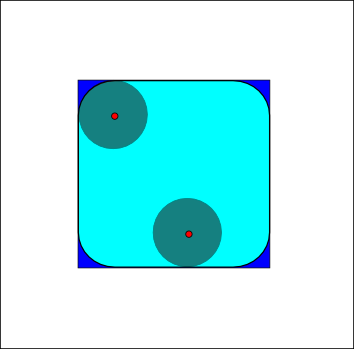
\includegraphics[width=0.25\textwidth]{img/Opening}  \\
    
\includegraphics[width=0.35\textwidth]{img/opening2} 
      \caption{Quelle: Wikipedia, OpenCV}
\end{figure}

 \end{frame}
\begin{frame}
    \frametitle{Morphologische Filter}
\framesubtitle{}

\begin{figure}[htp]
      \centering
Closing \\
    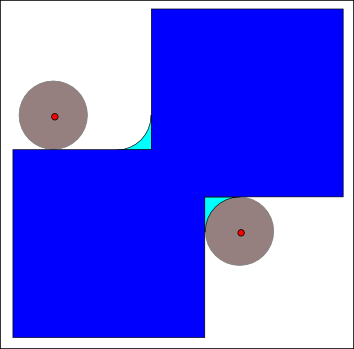
\includegraphics[width=0.25\textwidth]{img/Closing}  \\
    
\includegraphics[width=0.35\textwidth]{img/closing2} 
      \caption{Quelle: Wikipedia, OpenCV}
\end{figure}

 \end{frame}



\begin{frame}
    \frametitle{Morphologische Filter}
\framesubtitle{}

\begin{block}{Hit-or-miss Operator}
Seien $B,C \subset \mathbb{R}^n$ eine (nichtleere) Teilmenge und $u : \mathbb{R}^n \to \{ 0,1 \}$  eine binäres Bild. Dann ist der  Hit-or-Miss Operator definiert durch   
\begin{align*}
u   \odot (B,C) := (u \ominus B) \wedge (u^c \ominus C)
\end{align*}
Für ein Grauwertbild $u : \mathbb{R}^n \to [0,1]$ definiert man analog
\begin{align*}
u   \odot (B,C) := (u \ominus B) \cdot \bigl((1-u) \ominus C\bigr)
\end{align*}
\end{block}

 \end{frame}


\begin{frame}
    \frametitle{Morphologische Filter}
\framesubtitle{}

\begin{figure}[htp]
      \centering
    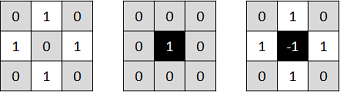
\includegraphics[width=0.45\textwidth]{img/hom1}  \\
    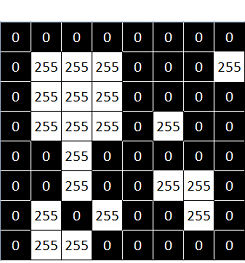
\includegraphics[width=0.35\textwidth]{img/hom2}   \; \; 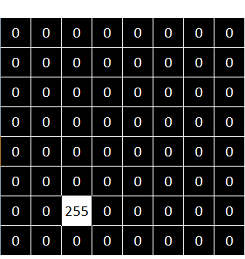
\includegraphics[width=0.35\textwidth]{img/hom3} 
      \caption{Quelle: OpenCV}
\end{figure}

 \end{frame}


\begin{frame}
    \frametitle{Kantenerkennung nach Canny}
\framesubtitle{}

\begin{block}{Kantenerkennung mit Hilfe von Gradienten}
Eine Kante weisst eine hohe Änderung des Kontrastes und damit einen grossen Gradienten auf. Um grosse Gradienten zu vermeiden, die durch Rauschen verursacht werden, möchte wir das Bild vorher glätten. Doch welcher Filter ist hierfür Optimal?
 
\end{block}

 \end{frame}

\begin{frame}
    \frametitle{Kantenerkennung nach Canny}
\framesubtitle{}

\begin{block}{Kantenerkennung mit Hilfe von Gradienten}
Nehmen wir an, die gesuchte  Filterfunktion $f_\sigma$ hängt von einem Parameter $\sigma$ ab  und wir betrachten das gefilterte Bild $u(x, \sigma) := u(x) *f_\sigma (x)$.
 \begin{align*}
\frac{d}{d} u * f_s
\end{align*}
\href{https://www.youtube.com/watch?v=ToIXSwZ1pJU}{LINK}
\end{block}
 \end{frame}




\end{document}
